%Nous définissons ici chacunes des figures, appelées comme des fonctions dans les autres documents.

\newcommand{\Grilleblank}{
    \draw[thick] (0,0) rectangle (5,7);
    \draw[step=1cm] (0,0) grid (5,7);
    \foreach \x in {0,...,4}
        \foreach \y in {0,...,6}
            \fill(\x+0.5, \y+0.5) circle(2pt);
    \fill(2.5, 3.5) circle(2pt) node[fill opacity=0, text opacity=1, above] {$\mathbf{C}$};
}

\newcommand{\distanceq}{
    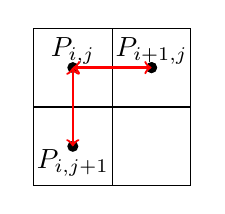
\begin{tikzpicture}[baseline=(midpoint)]
    \coordinate (midpoint) at (0,1);
    \draw[step=1cm] (0,0) grid (2,2);
    \fill(0.5, 0.5) circle(2pt) node[below] at (0.5,0.58) {$P_{i,j+1}$};
    \fill(0.5, 1.5) circle(2pt) node[above] at (0.5,1.42) {$P_{i,j}$};
    \fill(1.5, 1.5) circle(2pt) node[above] at (1.5,1.42) {$P_{i+1,j}$};
    \fill(1.5, 1.5) circle(2pt);
    \draw[<->, red, thick] (0.5,0.5) -- (0.5,1.5);
    \draw[<->, red, thick] (0.5,1.5) -- (1.5,1.5);
    \end{tikzpicture}
}

\newcommand{\screenrepresentation}{
    \tdplotsetmaincoords{110}{55}
    \begin{tikzpicture}[scale=4, tdplot_main_coords]
    \tikzset{fortext/.style={
        fill=white, fill opacity=0.5, text opacity=1, rounded corners
    }}
    %axis
    \filldraw[red] (0,0,0) circle(1pt) node[anchor=north east] {$\mathbf{E}$};
    \draw[->, red, very thick] (0,0,0) -- (1,0,0) node[black, anchor=west] {$\mathbf{C}$};
    \draw[->, red, very thick] (0,0,0) -- (0,1,0) node[anchor=south] {$\vec{r}$};
    \draw[->, red, very thick] (0,0,0) -- (0,0,1) node[anchor=north east] {$\vec{u}$};
    %camera
    \coordinate (A) at (-0.8, -0.15, -0.15);
    \coordinate (B) at (-0.8, -0.15, 0.15);
    \coordinate (C) at (-0.8,  0.15, 0.15);
    \coordinate (D) at (-0.8,  0.15, -0.15);
    \coordinate (E) at (0, -0.15,  -0.15);
    \coordinate (F) at (0, -0.15,  0.15);
    \coordinate (G) at (0,  0.15,  0.15);
    \coordinate (H) at (0,  0.15, -0.15);

    \draw (A) -- (B) -- (C) -- (D) -- cycle;
    \draw (E) -- (F) -- (G) -- (H) -- cycle;
    \draw (A) node[below] {camera} -- (E);
    \draw (B) -- (F);
    \draw (C) -- (G);
    \draw (D) -- (H);

    %ray vectors
    \pgfmathsetmacro{\qx}{1/(3*sqrt(3))}; %la valeur de qx est egale a celle de qy ici
    \foreach \i in {1,...,7} {
        \foreach \j in {1,...,5} {
            \draw[gray, ->] (0,0,0) -- 
            (1,{(\j-1)*(\qx)-(2*\qx)},{(\i-1)*(\qx)-(3*\qx)});
            \draw[fill] (1,{(\j-1)*(\qx)-(2*\qx)},{(\i-1)*(\qx)-(3*\qx)}) circle [radius=0.4pt];
        }
    }

    %Grille
    \path (1,-{(5/2)*\qx},-{(7/2)*\qx}) coordinate (start);
    \foreach \i in {0,...,5} {
        \draw[thick] ($(start)+(0,{\i*\qx},0)$) -- ($(start)+(0,{\i*\qx},{(7*\qx)})$) ;
    }
    \foreach \i in {0,...,7} {
        \draw[thick] ($(start)+(0,0,{\i*\qx})$) -- ($(start)+(0,{(5*\qx)},{\i*\qx})$) ;
    }

    \end{tikzpicture}
}

\newcommand{\stretched}{
    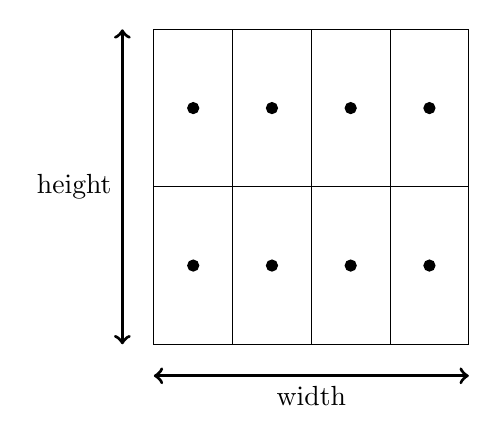
\begin{tikzpicture}[scale=2]
        \draw (0,0) rectangle (2,2);
        \draw[<->, very thick] (0,-0.2) -- (2,-0.2) node[below, midway] {width};
        \draw[<->, very thick] (-0.2,0) -- (-0.2,2) node[left, midway] {height};
        \draw (0,1) -- (2,1);
        \draw (0.5,0) -- (0.5,2);
        \draw (1,0) -- (1,2);
        \draw (1.5,0) -- (1.5,2);
        \foreach \x in {0.25,0.75,1.25,1.75} {
            \draw[fill] (\x,0.5) circle (1pt);
            \draw[fill] (\x,1.5) circle (1pt);
        }
    \end{tikzpicture}
}

\newcommand{\unstretched}{
    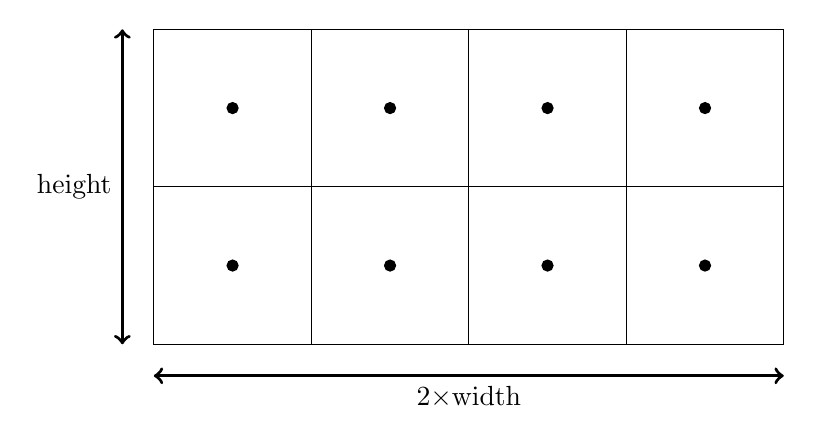
\begin{tikzpicture}[scale=2]
        \draw (0,0) rectangle (4,2);
        \draw[<->, very thick] (0,-0.2) -- (4,-0.2) node[below, midway] {2$\times$width};
        \draw[<->, very thick] (-0.2,0) -- (-0.2,2) node[left, midway] {height};
        \draw (0,1) -- (4,1);
        \draw (1,0) -- (1,2);
        \draw (2,0) -- (2,2);
        \draw (3,0) -- (3,2);
        \foreach \x in {0.5,1.5,2.5,3.5} {
            \draw[fill] (\x,0.5) circle (1pt);
            \draw[fill] (\x,1.5) circle (1pt);
        }
    \end{tikzpicture}
}

\newcommand{\triangles}{
    \tdplotsetmaincoords{110}{55}
    \begin{tikzpicture}[scale=4, tdplot_main_coords]
    \tikzset{fortext/.style={
        fill=white, fill opacity=0.5, text opacity=1, rounded corners
    }}
    \pgfmathsetmacro{\qx}{1/(3*sqrt(3))};

    %camera
    \coordinate (A) at (-0.8, -0.15, -0.15);
    \coordinate (B) at (-0.8, -0.15, 0.15);
    \coordinate (C) at (-0.8,  0.15, 0.15);
    \coordinate (D) at (-0.8,  0.15, -0.15);
    \coordinate (E) at (0, -0.15,  -0.15);
    \coordinate (F) at (0, -0.15,  0.15);
    \coordinate (G) at (0,  0.15,  0.15);
    \coordinate (H) at (0,  0.15, -0.15);

    \draw (A) -- (B) -- (C) -- (D) -- cycle;
    \draw (E) -- (F) -- (G) -- (H) -- cycle;
    \draw (A) node[below, fortext] {camera} -- (E);
    \draw (B) -- (F);
    \draw (C) -- (G);
    \draw (D) -- (H);

    %Grille
    \draw[<->, very thick] ($(start)+(0,{5*\qx+0.05},0)$) -- ($(start)+(0,{5*\qx+0.05},{7*\qx})$) node[right, midway, fortext] {height};

    \path (1,-{(5/2)*\qx},-{(7/2)*\qx}) coordinate (start);
    \foreach \i in {0,...,5} {
        \draw[thick] ($(start)+(0,{\i*\qx},0)$) -- ($(start)+(0,{\i*\qx},{(7*\qx)})$) ;
    }
    \foreach \i in {0,...,7} {
        \draw[thick] ($(start)+(0,0,{\i*\qx})$) -- ($(start)+(0,{(5*\qx)},{\i*\qx})$) ;
    }

    %triangles
    \shadedraw[right color=orange!80!white, left color=gray, draw=orange!50!black, fill opacity=0.6] (0,0,0) -- (1,0,0) -- (1,0,{3.5*\qx}) -- cycle;
    \draw[<->, very thick, blue!80!black] (1,0,0) -- (1,0,{3.5*\qx}) node[right, midway, fortext] {$tan(\dfrac{\theta}{2})$};
    \shadedraw[right color=green!80!white, left color=gray, draw=green!50!black, fill opacity=0.6] (0,0,0) -- (1,0,0) -- (1,0,-{3.5*\qx}) -- cycle;
    \draw[<->, very thick, blue!80!white] (1,0,0) -- (1,0,-{3.5*\qx}) node[right, pos=0.3, fortext] {$tan(\dfrac{\theta}{2})$};

    %axis
    \filldraw[red] (0,0,0) circle(1pt) node[anchor=north east, fortext] {$\mathbf{E}$};
    \draw[->, red, very thick] (0,0,0) -- (1,0,0) node[black, anchor=west, fortext] {$\mathbf{C}$};
    \draw[->, red, very thick] (0,0,0) -- (0,1,0) node[anchor=south, fortext] {$\vec{r}$};
    \draw[->, red, very thick] (0,0,0) -- (0,0,1) node[anchor=north east, fortext] {$\vec{u}$};
    \draw[fill] (1,0,0) circle [radius=0.4pt];

    \end{tikzpicture}
}

\newcommand{\paritee}{
    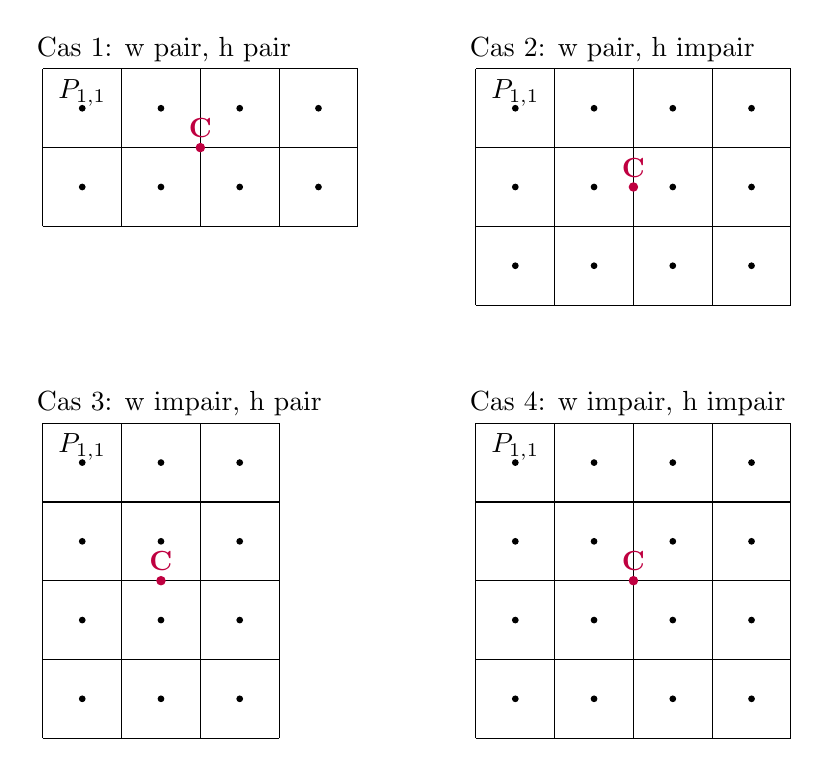
\begin{tikzpicture}
    \node[right] at (-0.2,0.25) {Cas 1: w pair, h pair};
    \draw[step=1] (0,0) grid (4,-2);
    \foreach \x in {0.5,1.5,2.5,3.5} {
        \draw[fill] (\x,-0.5) circle (1pt);
        \draw[fill] (\x,-1.5) circle (1pt);
    }
    \draw[fill, purple] (2,-1) node[above] {$\mathbf{C}$} circle (1.5pt);
    \node[above] at (0.5,-0.6) {$P_{1,1}$};

    \begin{scope}[shift={(5.5,0)}]
        \node[right] at (-0.2,0.25) {Cas 2: w pair, h impair};
        \draw[step=1] (0,0) grid (4,-3);
        \foreach \x in {0.5,1.5,2.5,3.5} {
            \draw[fill] (\x,-0.5) circle (1pt);
            \draw[fill] (\x,-1.5) circle (1pt);
            \draw[fill] (\x,-2.5) circle (1pt);
        }
        \draw[fill, purple] (2,-1.5) node[above] {$\mathbf{C}$} circle (1.5pt);
        \node[above] at (0.5,-0.6) {$P_{1,1}$};
    \end{scope}

    \begin{scope}[shift={(0,-4.5)}]
        \node[right] at (-0.2,0.25) {Cas 3: w impair, h pair};
        \draw[step=1] (0,0) grid (3,-4);
        \foreach \x in {0.5,1.5,2.5} {
            \draw[fill] (\x,-0.5) circle (1pt);
            \draw[fill] (\x,-1.5) circle (1pt);
            \draw[fill] (\x,-2.5) circle (1pt);
            \draw[fill] (\x,-3.5) circle (1pt);
        }
        \draw[fill, purple] (1.5,-2) node[above] {$\mathbf{C}$} circle (1.5pt);
        \node[above] at (0.5,-0.6) {$P_{1,1}$};
    \end{scope}

    \begin{scope}[shift={(5.5,-4.5)}]
        \node[right] at (-0.2,0.25) {Cas 4: w impair, h impair};
        \draw[step=1] (0,0) grid (4,-4);
        \foreach \x in {0.5,1.5,2.5,3.5} {
            \draw[fill] (\x,-0.5) circle (1pt);
            \draw[fill] (\x,-1.5) circle (1pt);
            \draw[fill] (\x,-2.5) circle (1pt);
            \draw[fill] (\x,-3.5) circle (1pt);
        }
        \draw[fill, purple] (2,-2) node[above] {$\mathbf{C}$} circle (1.5pt);
        \node[above] at (0.5,-0.6) {$P_{1,1}$};
    \end{scope}
    \end{tikzpicture}
}